% !TeX spellcheck = de_CH
%%%%%%%%%%%%%%%%%%%%%%%%%%%%%%%%%%%%%%%%%%%%%%%%%%%%%%%%%%%%%%%%%
%  _____   ____  _____                                          %
% |_   _| /  __||  __ \    Institute of Computitional Physics   %
%   | |  |  /   | |__) |   Zuercher Hochschule Winterthur       %
%   | |  | (    |  ___/    (University of Applied Sciences)     %
%  _| |_ |  \__ | |        8401 Winterthur, Switzerland         %
% |_____| \____||_|                                             %
%%%%%%%%%%%%%%%%%%%%%%%%%%%%%%%%%%%%%%%%%%%%%%%%%%%%%%%%%%%%%%%%%
%
% Project     : BA Welti Keller
% Title       : 
% File        : anhang.tex Rev. 00
% Date        : 15.09.2014
% Author      : Tobias Welti
%
%%%%%%%%%%%%%%%%%%%%%%%%%%%%%%%%%%%%%%%%%%%%%%%%%%%%%%%%%%%%%%%%%


\pagenumbering{Roman}

\appendix
\chapter{Anhang}\label{chap.anhang}

\todo{Anhang}

\section{Offizielle Aufgabenstellung}\label{app.aufgabenstellung}
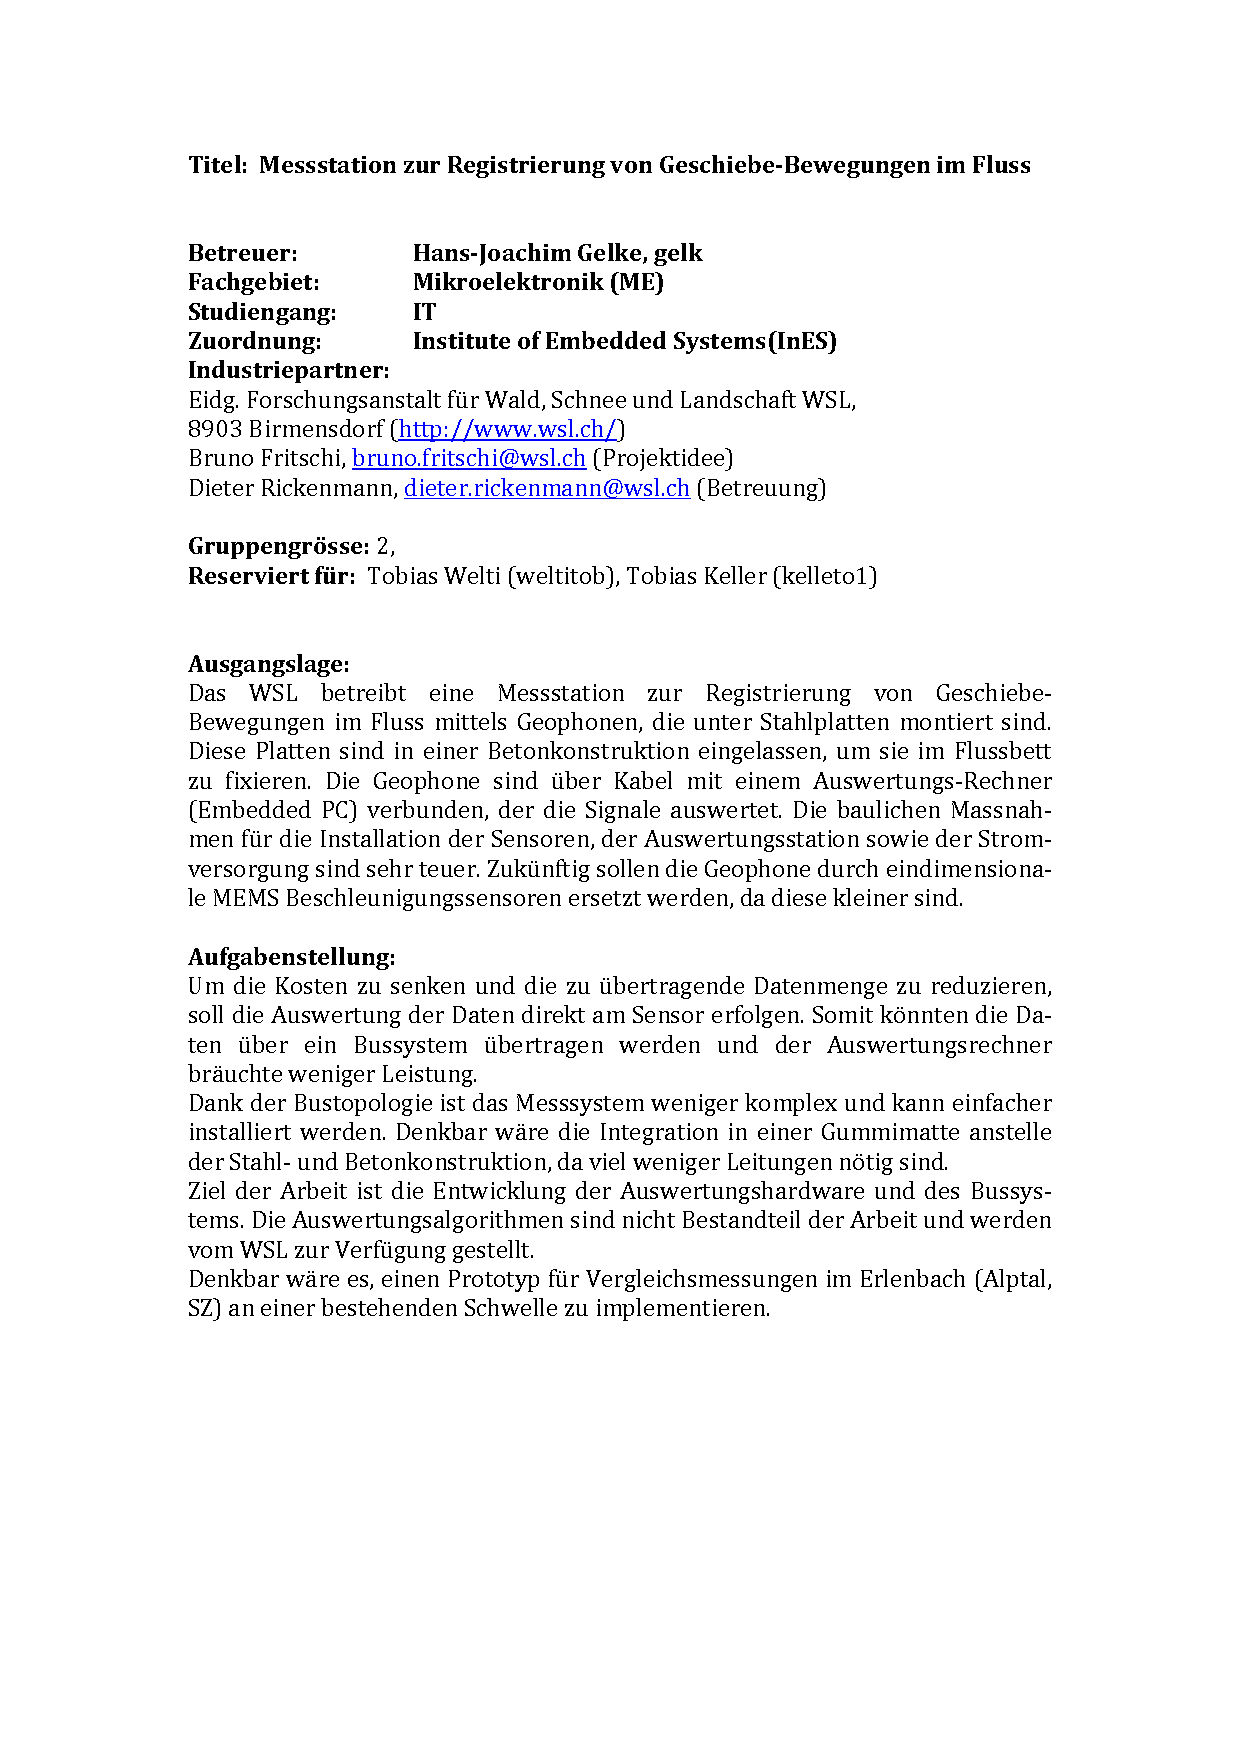
\includepdf{images/BA_welti_keller_hs14.pdf}


\section{Projektmanagement}\label{app.projektmanagement}


\todo{Zeitplan\\
Besprechungsprotokolle oder Journals}




\section{Weiteres}\label{weiteres}


\section{Schaltpläne}\label{app.pcb}
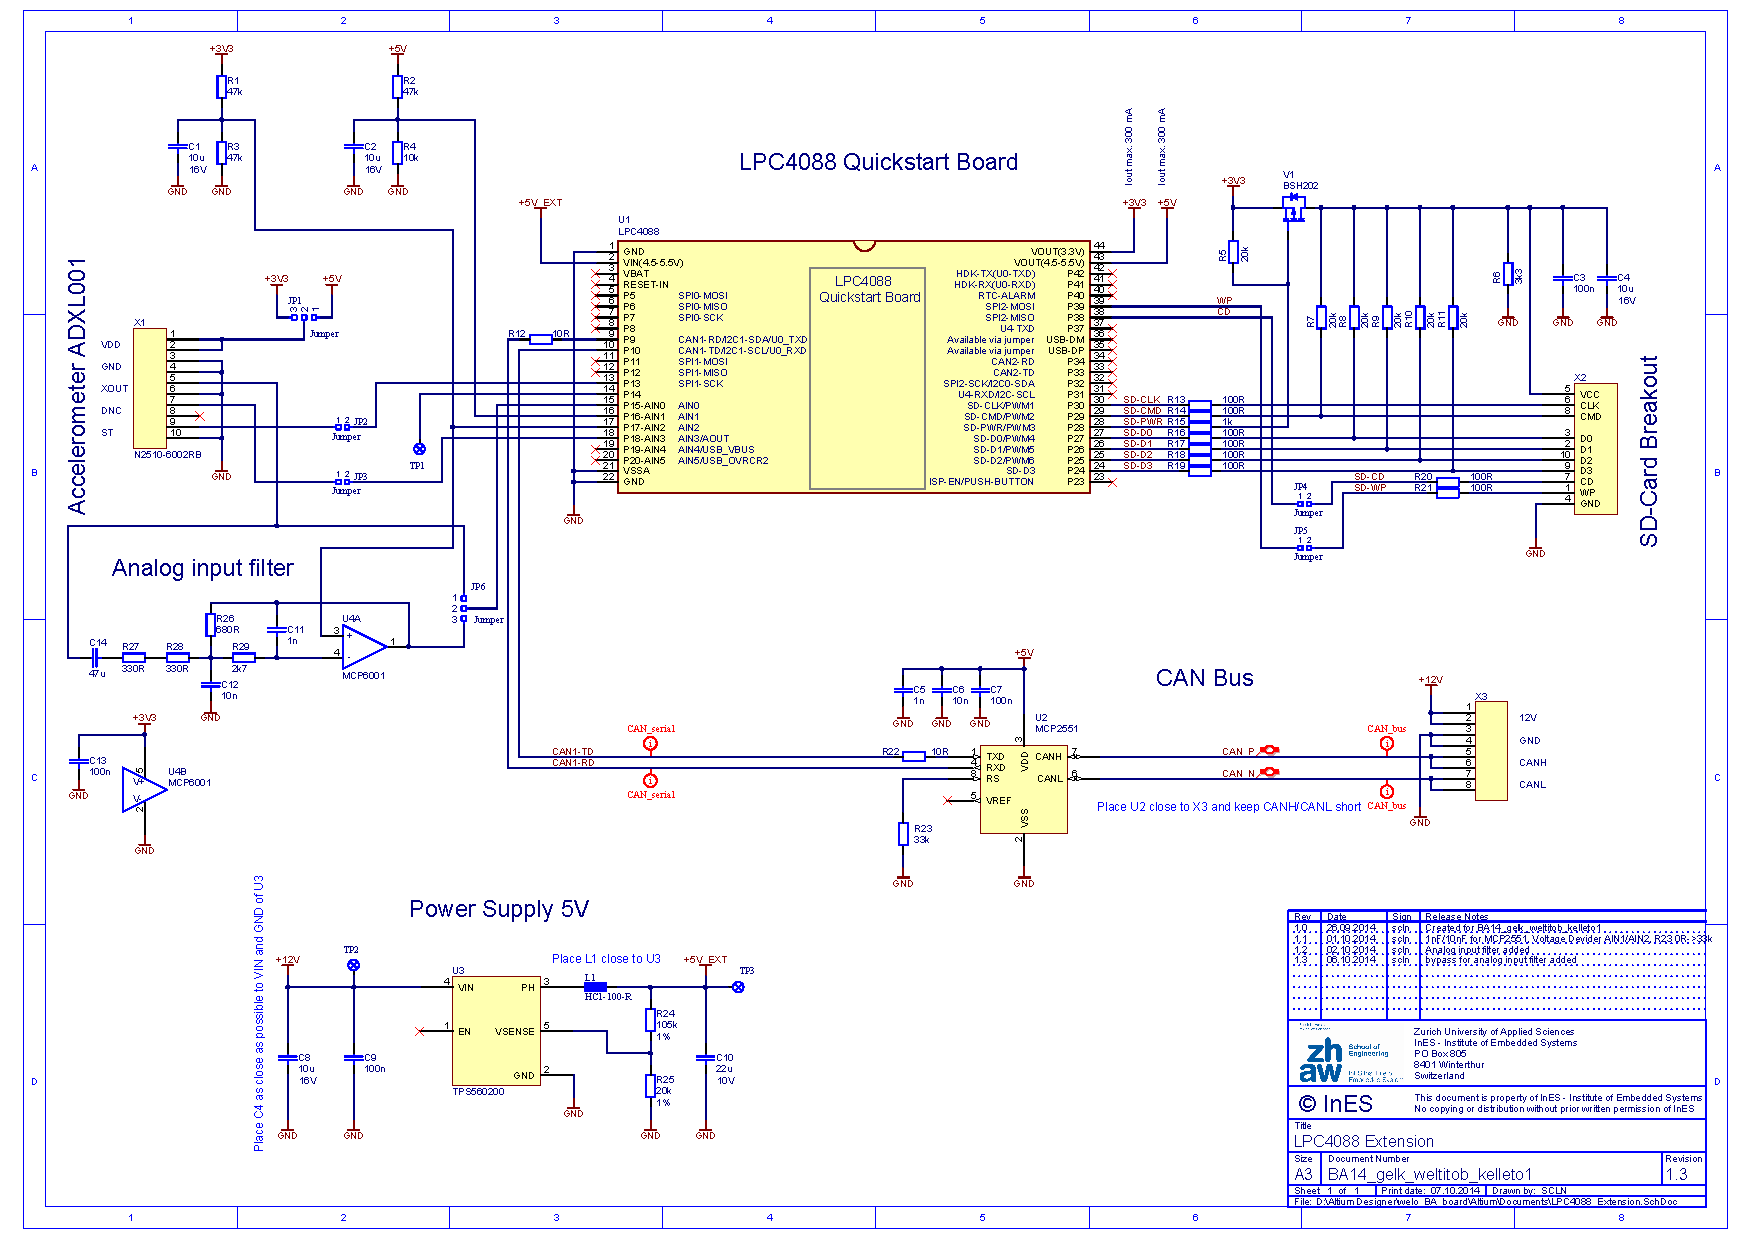
\includepdf[angle=90]{images/pcb/Schematic.pdf}
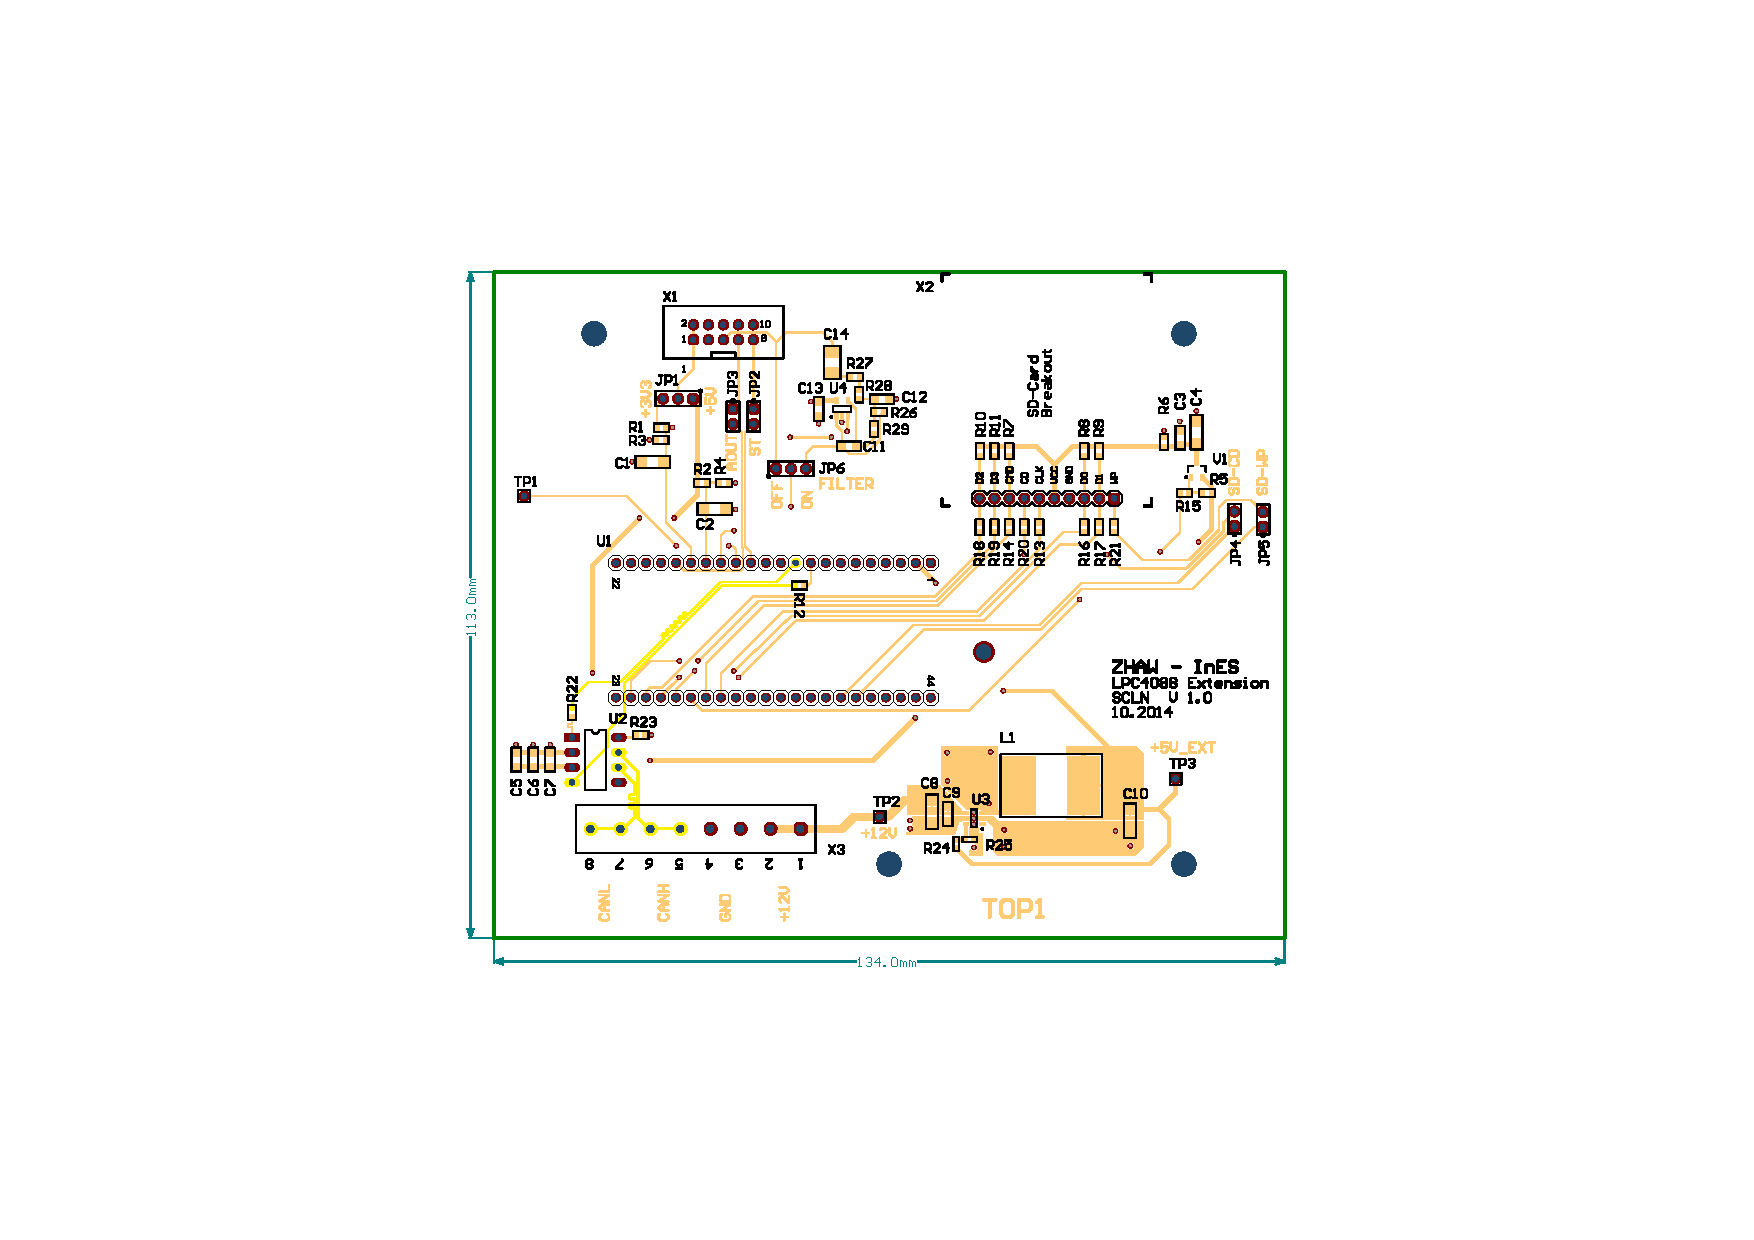
\includepdf[pages={1,2},angle=90]{images/pcb/PCB_Layout.pdf}


\section{Datenblätter}\label{app.datasheets}
Um die Dokumentation übersichtlich zu halten, wird der Grossteil der Datenblätter nicht mit der Dokumentation ausgedruckt, sondern auf der beiliegenden \gls{cd} mitgeliefert.


\subsection{NXP LPC4088 32-bit ARM Cortex-M4 microcontroller}
\includepdf[pages={7}]{images/datasheets/LPC408X_7X.pdf}\label{ds.lpc4088}


\subsection{Embedded Artists NXP LPC4088 QuickStart Board}

\begin{figure}[H]
	\centering		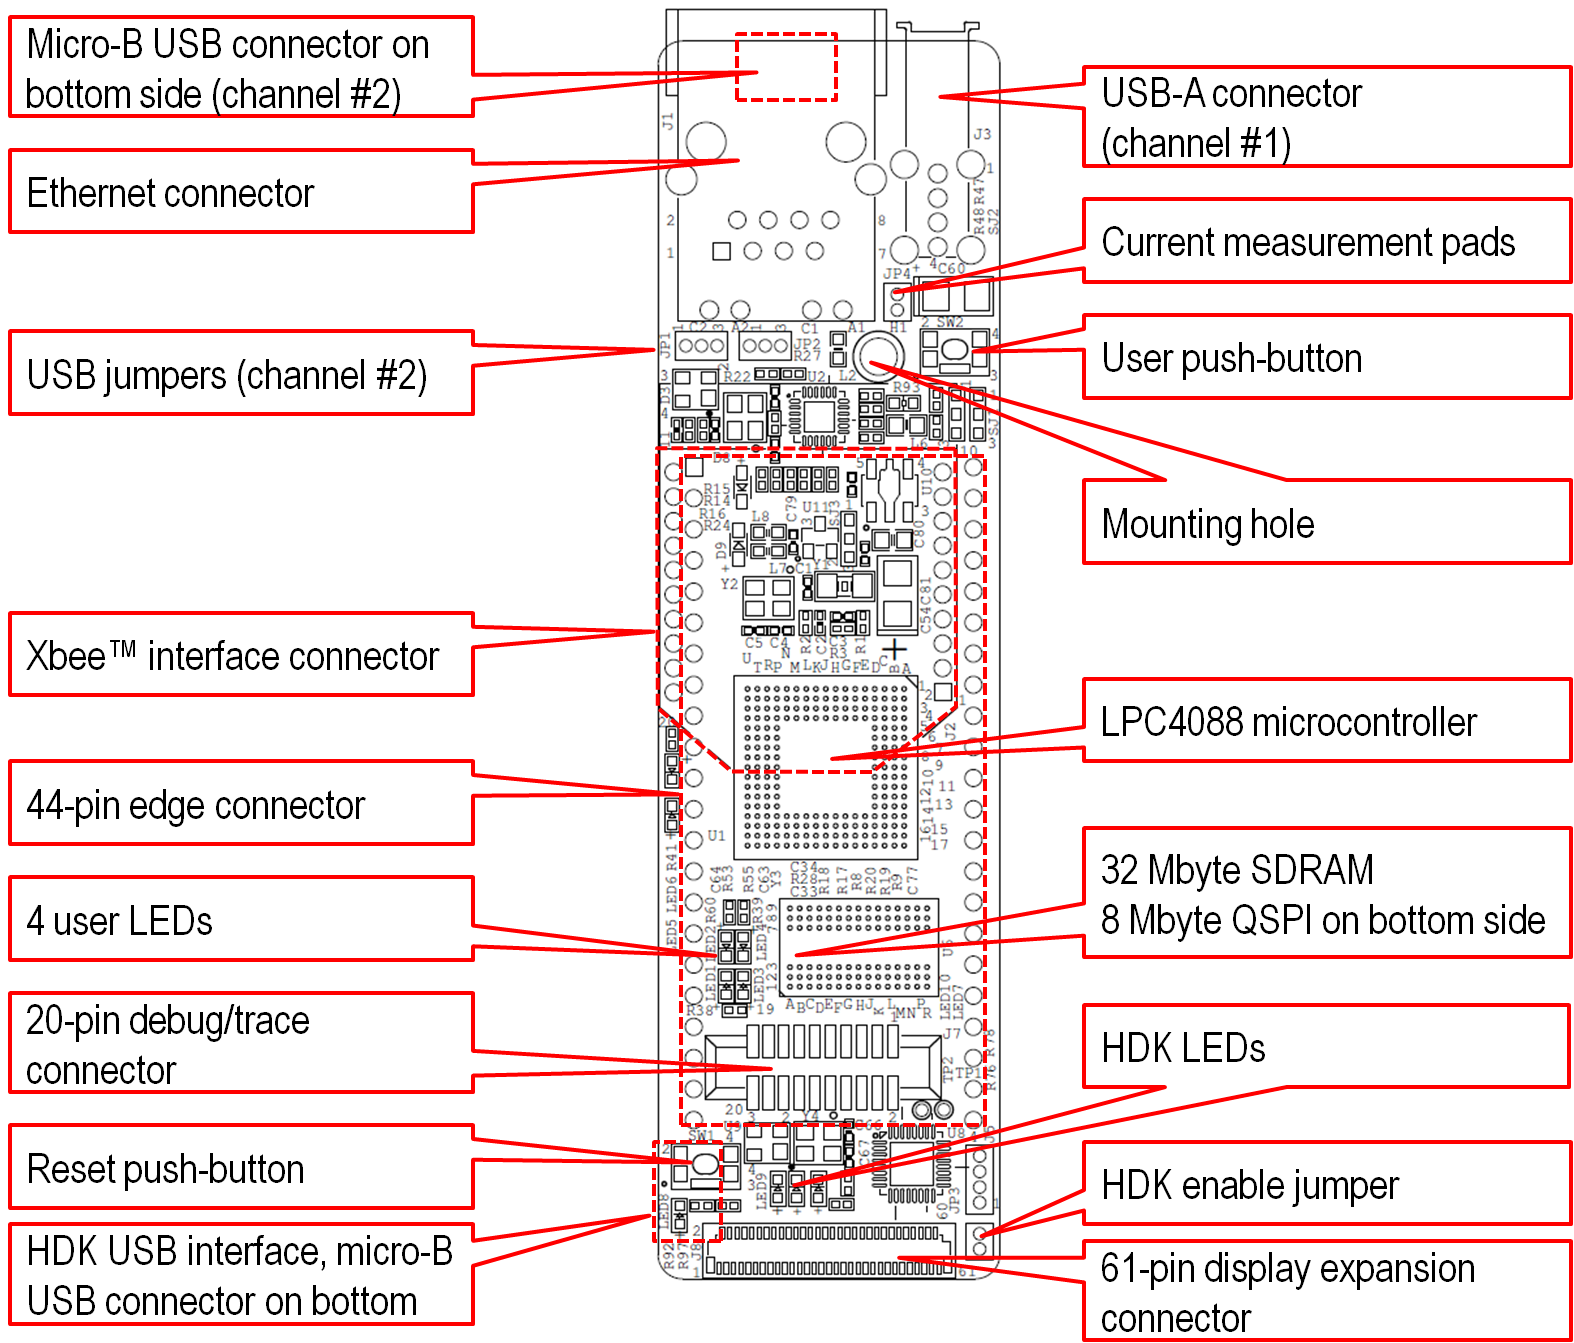
\includegraphics[width=0.7\textwidth]{images/datasheets/lpc4088_qsb_key_components_reva.png}
	\caption{Hauptkomponenten des NXP LPC4088 QuickStart Boards von Embedded Artists.}
	\label{fig.NXP_LPC4088_QSB_comps}
\end{figure}

\begin{figure}[H]
	\centering		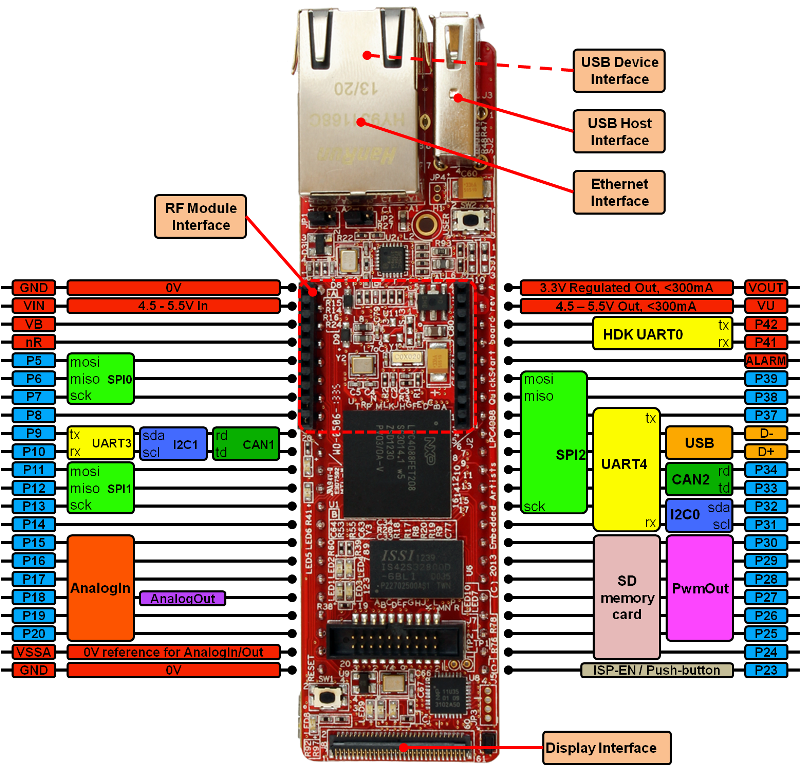
\includegraphics[width=0.7\textwidth]{images/datasheets/LPC4088_QSB_pinning_revA_800x769.png}
	\caption{Pins des NXP LPC4088 QuickStart Boards von Embedded Artists.}
	\label{fig.NXP_LPC4088_QSB_pinout}
\end{figure}

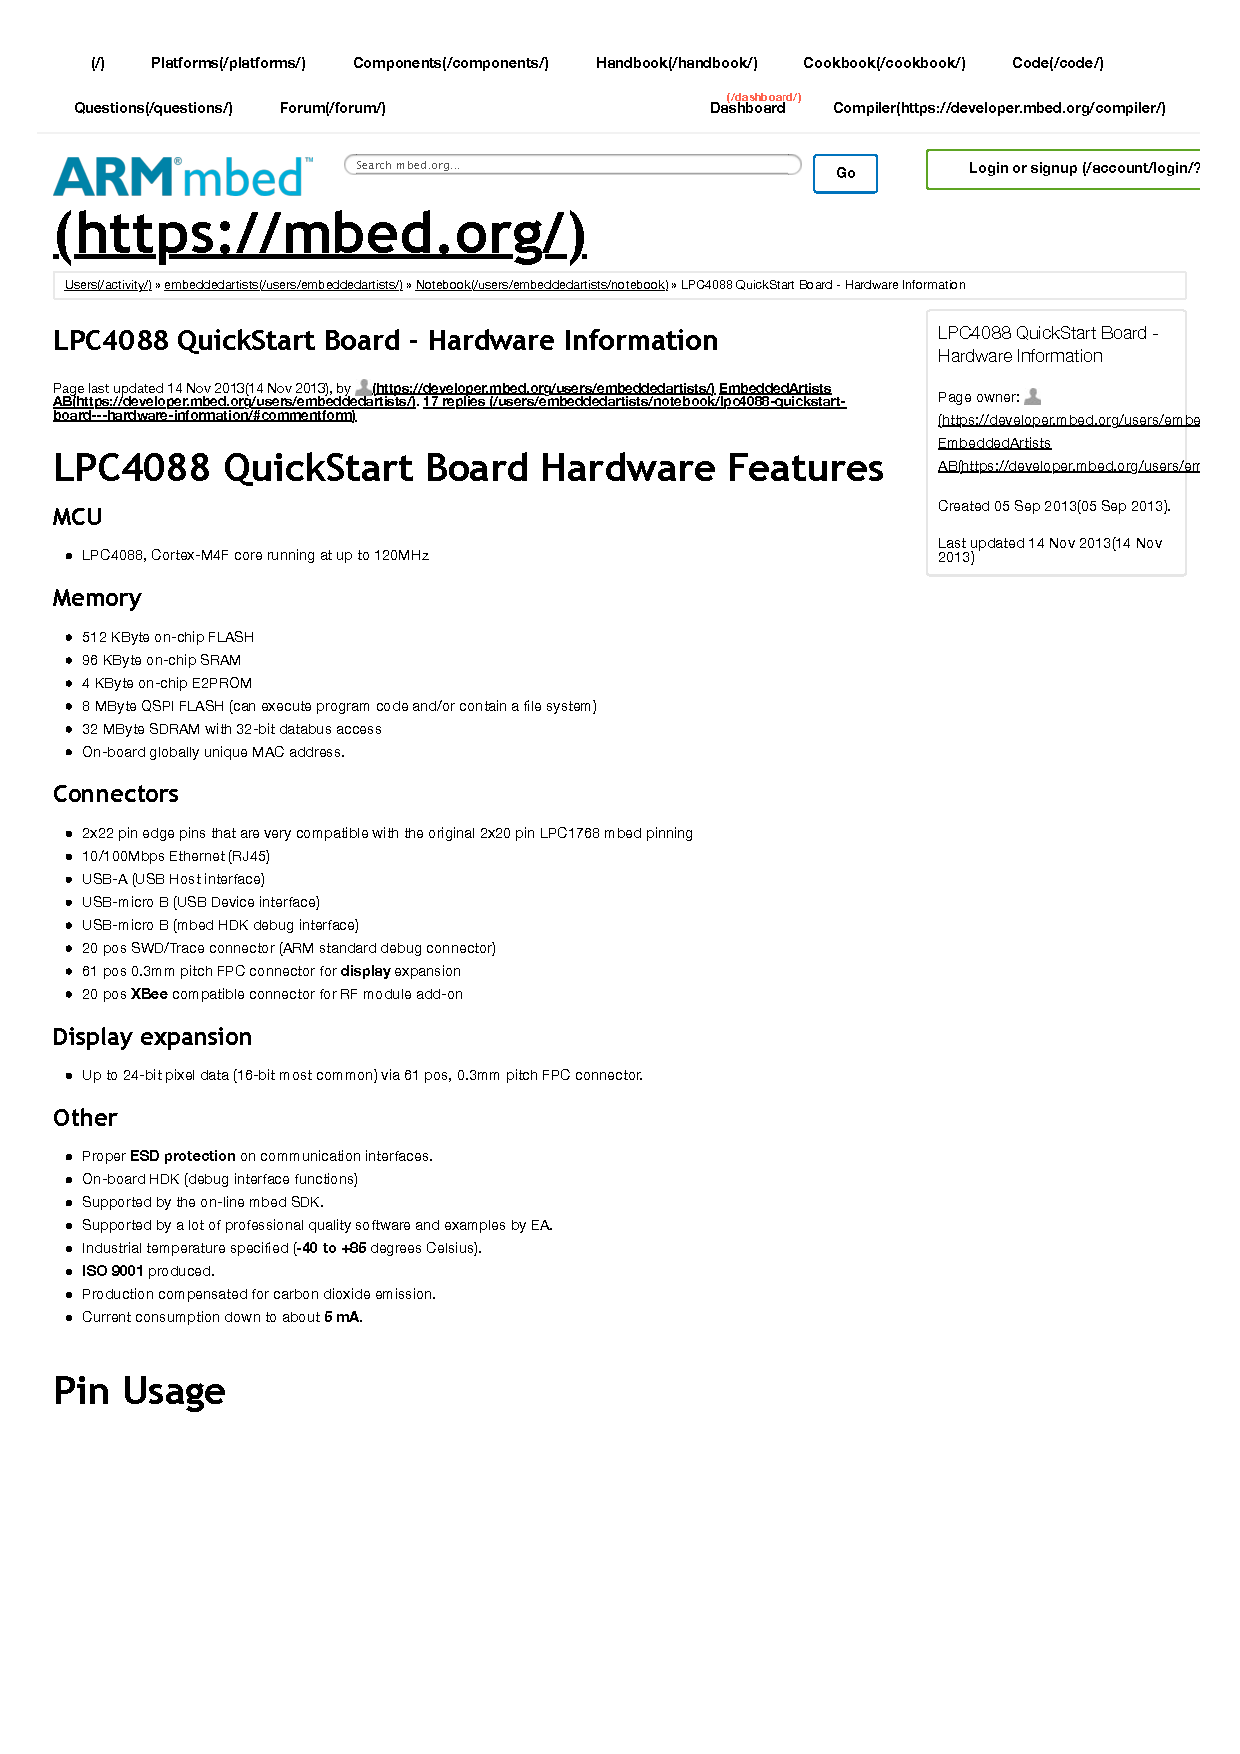
\includepdf{images/datasheets/LPC4088qsb.pdf}

\subsection{Analog Devices ADXL001 Beschleunigungssensor}
\includepdf[pages={3}]{images/datasheets/ADXL001.pdf}



\todo{Spezifikationen u. Datenblätter der verwendeten Messgeräte und/oder Komponenten\\
Berechnungen, Messwerte, Simulationsresultate\\
Grafische Darstellungen, Fotos}

\section{Source Code, Daten und Multimedia}\label{app.cd}
Da der Source Code sehr umfangreich ist, wird darauf verzichtet, ihn ausgedruckt zur Verfügung zu stellen. Er befindet sich auf der beiliegenden \gls{cd}.

\todo{Inhaltsverzeichnis der CD erstellen\\
CD mit dem vollständigen Bericht als pdf-File inklusive Film- und Fotomaterial}
